\documentclass[12pt]{article}
\title{Parsybone  manual}
\author{Adam Streck \\
		Systems Biology laboratory}
\usepackage{alltt}
\usepackage{a4wide}
\usepackage{pgf}
\usepackage{tikz}

%Environments used for description of DBM
\newenvironment{menum}{
\begin{enumerate}
  \setlength{\itemsep}{0pt}
  \setlength{\parskip}{0pt}
  \setlength{\parsep}{0pt}
}{\end{enumerate}}
\newenvironment{mitem}{
\begin{itemize}
  \setlength{\itemsep}{0pt}
  \setlength{\parskip}{0pt}
  \setlength{\parsep}{0pt}
}{\end{itemize}}

\begin{document}
\maketitle

\section{Introduction}
\subsection{Preface}
Parsybone is a CLI based tool for synthesis of discrete kinetic parameters in gene regulatory networks~\cite{TCBB2011} and their further analysis. Regulatory networks are provided using a so-called \emph{Thomas network} formalism~\cite{ThomasR1991} and analyzed using a method of \emph{colored} LTL model checking~\cite{TechReport}. The model checking procedure is based on the behavioral constrains provided in the form of B\"uchi automata~\cite{MCBible}. Features of this tool include:

\begin{itemize}
\item Reduction of the parameter space by application of edge constrains~\cite{TCBB2012}.
\item Enumeration of the shortest witnesses~\cite{TechReport} for synthesized parameters.
\item Enumeration of the \textrm{Robustness}~\cite{TechReport} values for synthesized parameters.
\item Computation in a distributed environment.
\end{itemize}

This manual describes the usage of the version $1.000$ of the tool and the version $1.0$ of the associate modeling language.

\subsection{Availability}
 The tool is freely available under the GNU GPLv3 license. The latest version of the tool can be obtained from the GitHub repository at https://github.com/sybila/Parsybone, the version described in this manual is available at https://github.com/sybila/Parsybone/tree/1.000. 

\subsection{Compiling Parsybone}
The only currently available version of the program is a source code archive, which has to be compiled before the tool can be run. For this a GNU C++ compiler of version at least 4.6.0 must be used (MinGW can serve as a replacement on the Windows platform).

To successfully compile the code you also need the Boost libraries~\cite{Boost} which can be obtained at http://www.boost.org/. The code has been tested using the 1.50.0 version.

The tool can be then compiled by invoking the GNU make utility in the main directory (the one containing the file \emph{Makefile}).

\section{Basics}
In this section we provide a concise introduction to the topic of the Thomas formalism, sufficient for understanding our modeling method and language. For more complex description of the Thomas formalism we would recommend the reader to refer to more elaborate articles, such as~\cite{ThomasR1991}. Readers well-established in the topic can skip this section alltogether.

To help with understanding of concepts of the Thomas formal method we demonstrate basic notions on a very simple example of a regulatory network, depicted in Figure~\ref{ExampNet}. This network has two boolean components named $0$ and $Y$, each regulated by both itself and the other component. This a bit unconventional naming has been choosen to demonstrate variability of modeling language later in the Section~\ref{sec:modeling}.

The model is a boolean one, which means that there are only two activity levels for each component, roughly corresponding to the situations where its concentration is below threshold or above it. The threshold marks a concentration boundary whose crossing usually causes the component to change its regulatory effect. Boolean component therefore usually works as a switch.

\begin{figure}[b]
\centering
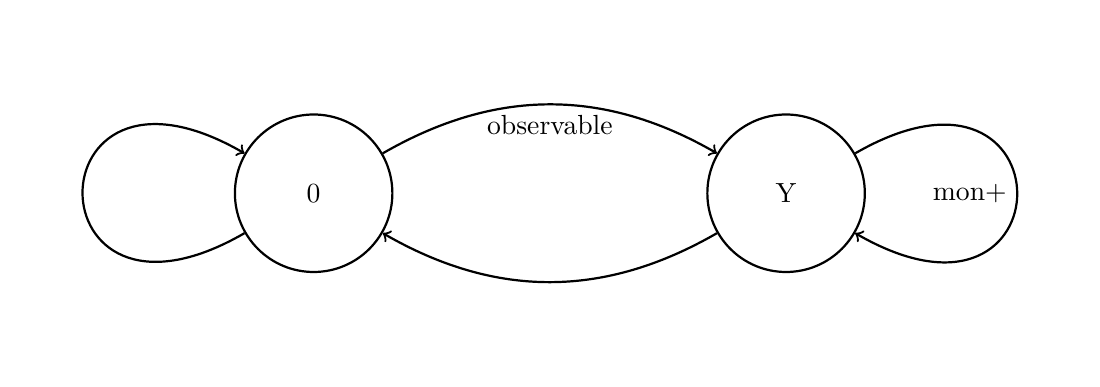
\begin{tikzpicture}
\node[draw, circle, thick, minimum size=20mm] (0) at (0,0) {0};
\node[draw, circle, thick, minimum size=20mm] (Y) at (6,0) {Y};
\draw[->, thick] (0) to [in=150,out=210,loop] (0);
\draw[->, thick] (0) to [bend left=30] node[below] {observable} (Y);
\draw[->, thick] (Y) to [bend left=30] (0);
\draw[->, thick] (Y) to [in=330,out=30,loop] node[left] {mon+} (Y);
\end{tikzpicture}
\caption{Simple example network with two components.}
\label{ExampNet}
\end{figure}

Components of such a network are usually well-know, conversely to their regulatory effects that are hard to obtain from biological measurements~\cite{Hecker09}. The Parsybone is designed to solve the task of determining those effects or at least to narrow the set of posibilities thus helping with further analysis. Possible regulatory effects of a component are given by the so-called \emph{logical parameters}. Each component has usually several logical parameters that specify towards which activity level the component inclines based on the current activity levels of its regulators e.g. a self-regulating component can stop its production when a certain concentration level is reached.

The user is required to specify the model as a set of components and their interactions. Having such a model, the Parsybone generates all possibile combinations of logical parameters for the model, creating a set of \emph{parametrizations}. This set is usually called \emph{parametrization space} and it can be viewed as a set of all behavioural possibilities for the model. As a second input, the Parsybone takes a specification of some behaviour the model must be able to reproduce. Parametrizations that do not allow such a behaviour are then removed from the set of possibilities.

Apart from basic boolean properties we also allow the model to be created using multiple extensions:
\begin{itemize}
\item Multi-valued components, allowing to change the effect of only a subset of its regulatory effects at a time.
\item Edge labels, bounding possible effects of the regulations.
\item Partial parametrizations, allowing to reduce the parametrization space before the analysis itself.
\item Basal values, specifying general case behaviour of components.
\end{itemize}

These extension allow for more precise model description than the basic boolean network formalism as presented above, but their explanation is beyond scope of this section. In case of furter interest please refer to~\cite{TechReport}.

\section{Modeling}
\label{sec:modeling}
 Models are described using an internal modeling language, based on the XML syntax~\cite{XML}, called \emph{DBM} (Discrete biological model). The model is provided within a single DBM file that holds specification for the model together with static and dynamic constrains of the parametrization space. Such a file has to have a \texttt{.dbm} suffix, and to abide by the overall rules for XML files.

\subsection{Model example}
Every model must be enclosed within a pair \texttt{MODEL} tag. This tag has a single mandatory attribute \texttt{ver}, which must contain a floating point number specifying the employed version of the DBM language. A detailed description of the whole language is provided later in this section, here we present, as an example, model file for the network depicted in Figure~\ref{ExampNet}. This example model has a quite non-uniform syntax, which has been chosen on purpose to present different possibilities of model description.
\begin{alltt}
<MODEL ver="1.0">
    <STRUCTURE>
        <SPECIE undef="basal">
            <REGUL source="1" threshold ="1" observ="1" />
            <REGUL source="0" />            
            <LOGIC formula="(Y &amp; !0)" />
        </SPECIE>
        <SPECIE name="Y">
            <REGUL source="0" />
            <REGUL source="Y" label="+" />            
            <PARAM context="" value="?" />
            <PARAM context="Y" value="1" />
            <PARAM context="0" value="0" />
            <PARAM context="0,1" />            
        </SPECIE>
    </STRUCTURE>
    ... specification of a property ...
</MODEL>
\end{alltt}
As can be seen, the model is a structure with two species, both being affected by two regulations. Formula $Y \wedge \neg 0$ gives the full parametrization of the component $0$. For the component $Y$, the possible parametrizations space is reduced by requirements that the regulation from $0$ must be observable and that the effect of its self-regulation must be positive, if any. Also, the logical parameter of self-regulation of the component $Y$ must always be 1. As a result, the parametrization space is reduced to four possibilities.

\subsection{Model property}
The main purpose of the tool is picking parametrizations that satisfy some property. The description of this property can be given in one of two possible ways - either as B\"uchi automaton or as a time series, whose specification is inserted between \texttt{</STRUCTURE>} and \texttt{</MODEL>} tags. A time series is merely a B\"uchi automaton specialization, but as will be explained later the Parsybone is optimized for its usage and provides additional features if the time series is employed. To demonstrate the difference between the two, we present a single property described using each formalism. This property assures that the model in Figure~\ref{ExampNet} is able to reproduce a time series composed of the following three measurements:
\begin{enumerate}
\item $0=0 \wedge (Y=0 \vee Y=1)$
\item $0 \Leftrightarrow Y$
\item $0=1 \wedge Y=0$
\end{enumerate}
Only two out of four parametrizations allow for reproduction of this time series. To obtain them, we can describe the time series either using the B\"uchi automaton:
\begin{alltt}
    <AUTOMATON>
        <STATE final="0">
            <EDGE target="0" label="tt" />
            <EDGE target="1" label="0=0" /> 
        </STATE>
        <STATE>
            <EDGE target="1" label="tt" />
            <EDGE target="last" label="((0=0 &amp; Y=0) | (0=1 &amp; 1=1))" /> 
        </STATE>
        <STATE name="last">
            <EDGE target="2" label="tt" />
            <EDGE target="3" label="(0=1 &amp; 1=0)" /> 
        </STATE>
        <STATE final="1">
            <EDGE target="4" label="tt" />
        </STATE>
    </AUTOMATON>
\end{alltt}
Or using the time series directly:
\begin{alltt}
    <SERIES>
        <EXPR values="0=0" />
        <EXPR values="((0=0 &amp; Y=0) | (0=1 &amp; 1=1))" />		
        <EXPR values="(0=1 &amp; Y=0)" />
    </SERIES>
\end{alltt}
As can be seen, the second method makes the model quite shorter and shuld be used for description of time series.

\subsection{Model holder description}
\begin{mitem}
	\item \texttt{MODEL}
	\begin{mitem}
		\item Occurrence: single, mandatory.
		\item Type: pair.
		\item Parent: none.
		\item Description: encloses the whole model.
		\item Attributes:	
		\begin{menum}
			\item \textit{ver} 
			\begin{mitem}
				\item Occurrence: mandatory.
				\item Value: must be $1.0$ in the current version of the tool.
			\end{mitem}
		\end{menum}
	\end{mitem}
\end{mitem}

\subsection{Regulatory network description}
\begin{mitem}
	\item \texttt{STRUCTURE}
	\begin{mitem}
		\item Occurrence: single, mandatory.
		\item Type: pair.
		\item Parent: MODEL.
		\item Description: encloses the definition of a regulatory network.
		\item Attributes: none.
	\end{mitem}
\end{mitem}
	
\begin{mitem}
	\item \texttt{SPECIE}
	\begin{mitem}
		\item Occurrence: multiple, mandatory.
		\item Type: pair.
		\item Parent: STRUCTURE.
		\item Description: defines a single specie.
		\item Attributes:	
		\begin{menum}
			\item \textit{name} 
			\begin{mitem}
				\item Occurrence: optional.
				\item Value: string containing letters and numbers.
				\item Default: ordinal number of the tag, counting from zero.
				\item Description: name of the specie under which it will be further addressed. System also uses its ordinal number (so the first specie can be addressed using the name \emph{0}).
			\end{mitem}
			\item \textit{undef} 
			\begin{mitem}
				\item Occurrence: optional.
				\item Value: basal/param/error.
				\item Default: param.
				\item Description: tells the system how it should handle values of regulatory contexts that are not specified. Basal means using a basal value, param means using all possible values and error causes error in case there are unspecified parameters.
			\end{mitem}
			\item \textit{max} 
			\begin{mitem}
				\item Occurrence: optional.
				\item Value: natural number.
				\item Default: 1.
				\item Description: maximal activation level this specie can occur in.
			\end{mitem}
			\item \textit{basal} 
			\begin{mitem}
				\item Occurrence: optional.
				\item Value: positive integer.
				\item Default: 0.
				\item Description: basal activation level of this specie - the value towards which the specie tends if not specified otherwise.
			\end{mitem}
		\end{menum}
	\end{mitem}
\end{mitem}

\begin{mitem}
	\item \texttt{REGUL}
	\begin{mitem}
		\item Occurrence: multiple, mandatory.
		\item Type: solo.
		\item Parent: SPECIE.
		\item Description: defines a single incoming regulation of the parent specie.
		\item Attributes:	
		\begin{menum}
			\item \textit{source} 
			\begin{mitem}
				\item Occurrence: mandatory.
				\item Value: name or the ordinal number of a specie.
				\item Description: name of the specie that regulates this one.
			\end{mitem}
			\item \textit{threshold} 
			\begin{mitem}
				\item Occurrence: optional.
				\item Value: natural number.
				\item Default: 1.
				\item Description: lowest activation level of the source specie that activates the regulation.
			\end{mitem}
			\item \textit{label} 
			\begin{mitem}
				\item Occurrence: optional.
				\item Value: + or - or ?.
				\item Default: ?.
				\item Description: describes nature of the regulation as activation (+) or inhibition (-) or any (?).
			\end{mitem}
			\item \textit{observ} 
			\begin{mitem}
				\item Occurrence: optional.
				\item Value: Boolean.
				\item Default: 0.
				\item Description: specifies if the regulation must be observable (1) or can be unobserved (0).
			\end{mitem}
		\end{menum}
	\end{mitem}
\end{mitem}
		
\begin{mitem}
	\item \texttt{PARAM}
	\begin{mitem}
		\item Occurrence: multiple, present if and only if there is no sibling LOGIC tag.
		\item Type: solo.
		\item Parent: SPECIE.
		\item Description: defines a single kinetic parameter.
		\item Attributes:	
		\begin{menum}
			\item \textit{context} 
			\begin{mitem}
				\item Occurrence: mandatory.
				\item Value: comma separated list of active regulations, given by a name or an ordinal number of a regulator.
				\item Description: defines the exact regulatory context in which this kinetic parameter is applied.
			\end{mitem}
			\item \textit{value} 
			\begin{mitem}
				\item Occurrence: optional.
				\item Value: positive integer or ?.
				\item Default: ?.
				\item Description: specifies target value of the specie in this regulatory context, which must be one of possible activation levels of the specie. Character ? means that an exact number is unknown and a parametrization for each value between 0 and the maximal activation level of the specie is created.
			\end{mitem}
		\end{menum}
	\end{mitem}
\end{mitem}
	
\begin{mitem}
	\item \texttt{LOGIC}
	\begin{mitem}
		\item Occurrence: single, present if and only if there is no sibling PARAM tag.
		\item Type: solo.
		\item Parent: SPECIE.
		\item Description: defines parametrization of the specie using a logical formula over the regulators.
		\item Attributes:	
		\begin{menum}
			\item \textit{formula} 
			\begin{mitem}
				\item Occurrence: mandatory.
				\item Value: logical formula (see Section~\ref{FormulaConstruction}), variables must be names or ordinal numbers of regulators.
				\item Description: result target value is given as a valuation of the formula, where a variable denoting a regulator is valuated to $1$ if the regulation is active and to $0$ otherwise.
			\end{mitem}
		\end{menum}
	\end{mitem}
\end{mitem}

\subsection{B\"uchi automaton description}		
\begin{mitem}
	\item \texttt{AUTOMATON}
	\begin{mitem}
		\item Occurrence: single, present if and only if there is no sibling SERIES tag.
		\item Type: pair.
		\item Parent: MODEL.
		\item Description: encloses decription of a B\"uchi automaton.
		\item Attributes: none.
	\end{mitem}
\end{mitem}		

\begin{mitem}
	\item \texttt{STATE}
	\begin{mitem}
		\item Occurrence: multiple, mandatory.
		\item Type: solo.
		\item Parent: AUTOMATON.
		\item Description: defines a single state of the automaton. The first state in the description is also considered to be the initial state of the automaton.
		\item Attributes: none.
	\end{mitem}
		\begin{menum}
			\item \textit{name} 
			\begin{mitem}
				\item Occurrence: optional.
				\item Value: string containing letters and numbers.
				\item Default: ordinal number of the tag, counting from zero.
				\item Description: name of the specie under which it will be further addressed. System also uses its ordinal number (so the first state can be addressed using the name \emph{0}).
			\end{mitem}
			\item \textit{final} 
			\begin{mitem}
				\item Occurrence: optional.
				\item Value: Boolean.
				\item Default: 0.
				\item Description: specifies if the state is final (1) or not (0).
			\end{mitem}
		\end{menum}
\end{mitem}		

\begin{mitem}
	\item \texttt{EDGE}
	\begin{mitem}
		\item Occurrence: multiple, mandatory.
		\item Type: solo.
		\item Parent: STATE.
		\item Description: defines an edge leading from the parent state.
		\item Attributes: 
		\begin{menum}
			\item \textit{target} 
			\begin{mitem}
				\item Occurrence: mandatory.
				\item Value: name or the ordinal number of the target state.
			\end{mitem}
			\item \textit{label} 
			\begin{mitem}
				\item Occurrence: mandatory.
				\item Value: logical formula (see Section~\ref{FormulaConstruction}), variables are atomic propositions (see Section~\ref{AtomicPropositions}).
				\item Description: conditions that must be met for the edge to be transitible.
			\end{mitem}
		\end{menum}
	\end{mitem}			
\end{mitem}		

\subsection{Time series description}
\begin{mitem}
	\item \texttt{SERIES}
	\begin{mitem}
		\item Occurrence: single,  present if and only if there is no sibling AUTOMATON tag.
		\item Type: pair.
		\item Parent: MODEL.
		\item Description: encloses definition of a time series.
		\item Attributes: none.
	\end{mitem}
\end{mitem}				
	
\begin{mitem}
	\item \texttt{EXPR}
	\begin{mitem}
		\item Occurrence: multiple, mandatory.
		\item Type: solo.
		\item Parent: SERIES.
		\item Description: a single measurement in the time series.
		\item Attributes:	
		\begin{menum}
			\item \textit{values} 
			\begin{mitem}
				\item Occurrence: mandatory.
				\item Value: logical formula (see Section~\ref{FormulaConstruction}), variables of the formula must be atomic propositions (see Section~\ref{AtomicPropositions}).
				\item Description: conditions that must be met for the measurement to be reproduced.
			\end{mitem}
		\end{menum}
	\end{mitem}
\end{mitem}	

\subsection{Formula construction}
\label{FormulaConstruction}
A formula is constructed using the following set of recursive rules:
\begin{enumerate}
\item $tt$ and $ff$ are formulas representing true or false respectively,
\item any variable is a formula,
\item for every formula $A$ is $\neg A$ a formula,
\item for formulas $A,B$ are $(A|B)$ and $(A\&B)$ formulas representing logical disjunction or conjunction respectively,
\item nothing else is a formula.
\end{enumerate}
Note that in the model $\neg$ is denoted using \texttt{!} and $\&$ is denoted using \texttt{\&amp;}.

\subsection{Atomic propositions}
\label{AtomicPropositions}
An atomic proposition is a string of the form: $specie*value$, where:
\begin{itemize}
\item $specie$ denotes the name or ordinal number of a specie,
\item $*$ denotes comparison operator from the set $\{<,>,=\}$,
\item $value$ denotes a positive integer with which the value of the specie is compared.
\end{itemize}
Note that in the model $<$ is denoted using \texttt{\&lt;} and $>$ is denoted using \texttt{\&gt;}.

\section{Usage}
Parsybone is a CLI-based tool and therefore all its settings are provided as text arguments when starting the tool - from that point on, there is no way to influence the process or its results. In this section we describe how and which arguments can be used and what results the computation process gives. It is also important to have in mind that the Parsybone is primarily designed for the time series analysis and some of its capabilities rely on its usage.

\subsection{Execution}
The syntax of the execution is:
\begin{alltt}
Parsybone 
    filename
    [-rsvwW]
    [-d num1 num2]
    [-f filename]
    [-m filename]
    [-M filename]
\end{alltt}
The first argument, $filename$, is the only one that must be present and it gives the name of a file containing the specification of a model and a property to be checked on that model. The file also has to have a \emph{.dbm} suffix, otherwise it will be rejected.

Other arguments tell the tool to alter the procedure somehow and their meaning is described in the following list. Techniques of their usage are explained in more detail later in this section.
\begin{itemize}
\item $-r$: for each feasible parametrization compute and display its \textrm{Robustness} value.
\item $-s$: display statistics during the computation (mainly sizes of graphs and parametrization sets used).
\item $-v$: display progress of individual parts of the computation.
\item $-w$: for each feasible parametrization compute and display transitions belonging to the shortest time series walks. Use numerical ID of states when describing transitions.
\item $-W$: similar to $-w$, but use full values of states instead. This switch has a higher priority than $-w$.
\item $-d$ $num1$ $num2$: test only a subspace of the parametrization space. This subspace is given as a $num1$-th part from $num2$ total parts.
\item $-f$ $filename$: store feasible parametrizations and their properties in the given file.
\item $-m$ $filename$: test only parametrizations marked in the provided file.
\item $-M$ $filename$: store mask of feasible parametrizations in the given file.
\end{itemize}

\subsection{Output format}
There are four types of internal streams that are used within the program:
\begin{itemize}
\item statistics: This stream is visible only when the $-s$ switch is used, it prints on a standard output stream and each of its lines starts with a \texttt{\#} symbol. This output contains mainly sizes of the structures and parametrizations sets used.
\item verbose: This stream is visible only when the $-v$ switch is used, it prints on a standard output stream and each of its lines starts with a \texttt{*} symbol. Independent parts of the process announce their start through this stream. It is mainly important because it displays progress of a coloring procedure.
\item errors: This stream prints on a standard error stream and each of its lines starts with a \texttt{!} symbol. Most error messages announce failure of the program.
\item results: This stream prints on a standard output stream or to a file provided using the $-f$ switch and it is the only stream whose lines have no prefix. The syntax of the content of this stream is described in the following section.
\end{itemize}

\subsection{Results syntax}
The result of the computation is a list of feasible parametrizations, one per line, possibly extended with an outcome of additional analysis. Each of the lines is in the following form: 
\texttt{ac\-cept\-able pa\-ra\-met\-riz\-a\-tion num\-ber}
\texttt{:}
\texttt{pa\-ra\-met\-riz\-a\-tion values}
\texttt{:}
\texttt{cost}
\texttt{:}
\texttt{ro\-bust\-ness}
\texttt{:}
\texttt{\{time se\-ries walks tran\-si\-tions\}}

Running an analysis of our example model using $-rW$ as an argument results in the following output:
\begin{alltt}
0:(0,1,0,0,0,0,1,0):3:0.5:\{(0,1;0)>(1,1;1),(1,1;1)>(1,0;2)\}
1:(0,1,0,0,1,0,1,0):3:0.5:\{(0,1;0)>(1,1;1),(1,1;1)>(1,0;2)\}
\end{alltt}

\subsection{Results semantics}
Each comma separated value represents some sort of information about the parametrization. The semantics of the independent values are defined as follows:
\begin{enumerate}
\item \texttt{ac\-cept\-able pa\-ra\-met\-riz\-a\-tion num\-ber}: this number uniquely identifies the pa\-ra\-met\-ri\-za\-tion within a set of all possible parametrizations of the model.
\item \texttt{pa\-ra\-met\-riz\-a\-tion values}: a vector of target values for each component. The values are ordered so that a parameter of the component that is closer to the beginning of the model file is before a parameter of the component that is closer to the end. The parameters of a single component are then ordered ascendingly by the number of present regulators. If the number is the same, contexts are again ordered by their appearance in the file. For our example model we first have the target value of the component $0$ with no present regulators, then with the self-regulation, then only with the regulation from the second component etc.
\item \texttt{cost}: The \textrm{Cost} value of this parametrizations given by a natural number. This value is only available for a time series property.
\item \texttt{ro\-bust\-ness}: The \textrm{Robustness} value of this parametrization given by a floating point number. This value is present only when the $-r$ switch has been used while checking a time series property.
\item \texttt{\{time se\-ries walks tran\-si\-tions\}}: A comma separated list of transitions corresponding to the shortest time series walks in the form \texttt{source>target}. 

If the $-W$ switch was used, this list contains a vector of current activation levels of each component, again ordered in the same manner as in which they are present in the model file, and the current state of the B\"uchi automaton separated by a semicolon. 

If the $-w$ switch was used, only the unique ID number of a state is used.

If neither $-w$ nor $-W$ were used or the property checked is not a time series, this part remains empty.
\end{enumerate}

\subsection{Using multiple properties}
It is possible to keep only parametrizations that satisfy multiple properties (this way for example bistability can be enforced). 
For this purpose, the tool must be run independently for each property that is to be tested and the underlying regulatory network must remain intact between computations so the parametrization spaces of the two match.
To save the information which parametrizations satisfy the property in a file, use the $-M$ switch followed by the name of the file to create. 
This file is then filled with a stream of bits where the $n$-th bit is set to $1$ if the $n$-th parametrization is feasible, otherwise it is set to $0$. This file can be read in a subsequent computation using the $-m$ switch - this ensures that only parametrizations that were marked as feasible are used.
It is also possible to create a chain of computations using both switches at once.

\subsection{Distribution}
Computation can be easily executed in a distributed environment - in such a case, the process does not take the whole parametrization space but only a part of it. This is done using the $-d$ switch with two numbers. The first number denotes the ID of this process and the second one the total number of processes employed - this tells the current process which part of the parametrization space it should use.

\subsection{Performance considerations}
There are some thoughts a user should keep in mind when creating a model to ensure its analysis is computable in reasonable time. The main performance issue is the size of parametrization space - adding new components is usually not a problem, but each new regulation increases the number of parametrizations of a single component greatly - a model that has a component with more than 5 regulators is not computable without any further reduction of the parametrization space (a boolean component with six regulators has roughly $2^{20}$ possible parametrizations). 

When checking a time series, the computation is much faster in comparison with standard $\omega$-regular property. This is due to the fact that this property belongs to the class of reachability properties that are much easier to check. On the other hand, computation of \textrm{Robustness} or shortest time series walks adds some overhead (if employed). These procedures rise in complexity with the length of the time series walk - the longer the distance between two successive measurements, the more complex this analysis gets - smaller differences between measurements or more precise definitions of measurements can help lower the complexity of these procedures.

\bibliographystyle{abbrv}
\bibliography{Manual}

\end{document}

% LocalWords:  Parsybone CLI LTL DBM GPLv GitHub MinGW GCC ver undef parametrizations REGUL observ PARAM EXPR param filename bistability reachability
